\documentclass[parskip]{article}
\usepackage[letterpaper, margin=1.25in]{geometry}
\usepackage{tikz}
\usepackage{float}
\usepackage{etoc}

\newlength\tocrulewidth
\setlength{\tocrulewidth}{1.5pt}

\usepackage{hyperref}
\hypersetup{
	colorlinks=true,
	linkcolor=blue,
	filecolor=magenta,      
	urlcolor=cyan,
}




\begin{document}


\setcounter{tocdepth}{1}
\tableofcontents

\pagebreak

\section{The model}

Here I will detail the math and implementation of the model. For now, here is a reference to what the section titles mean:

\begin{enumerate}
	\item \emph{Synapse Limit}: The maximum number of synapses each neuron can form.  
	\item \emph{Spatial Scale}: The coefficient that determines how sharply the probability of connection decreases with respect to distance between each pair of neurons
	\item \emph{Development Time}: The number of iterations that the network was allowed to run and form connections.
\end{enumerate}

\pagebreak

\foreach \s in {1,2,3}
{
\section{Synapse Limit: \s00}
\setcounter{tocdepth}{2}

\begingroup
\parindent=0em
\etocsettocstyle{\rule{\linewidth}{\tocrulewidth}\vskip0.5\baselineskip}{\rule{\linewidth}{\tocrulewidth}}
\localtableofcontents 
\endgroup


\pagebreak

\foreach \x in {05, 10,20,40}
	{ 
		\foreach \y in {10, 40, 70,100,140,180,200,220}
			{

			\subsection{Spatial Scale=\x , Development Time=\y}
				
			\begin{figure}[H]
			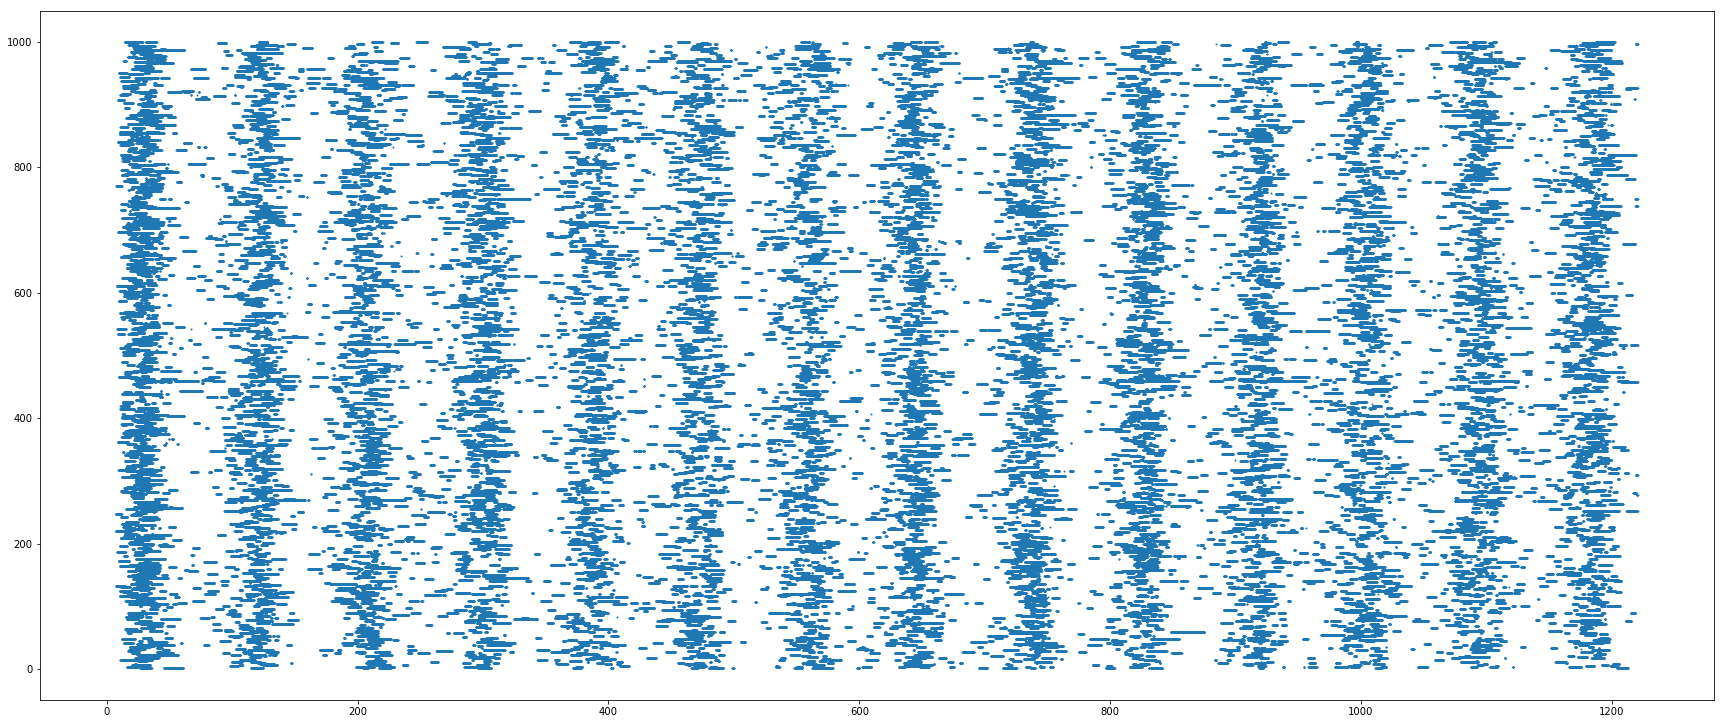
\includegraphics[width=1\linewidth,height=7cm]{/Users/sahand/Research/NeuroNet/Data/BW\s/N1000L\s00S\x D\y/Vis/TimeFrequency.png}
			\end{figure}
		
			\begin{figure}[H]
			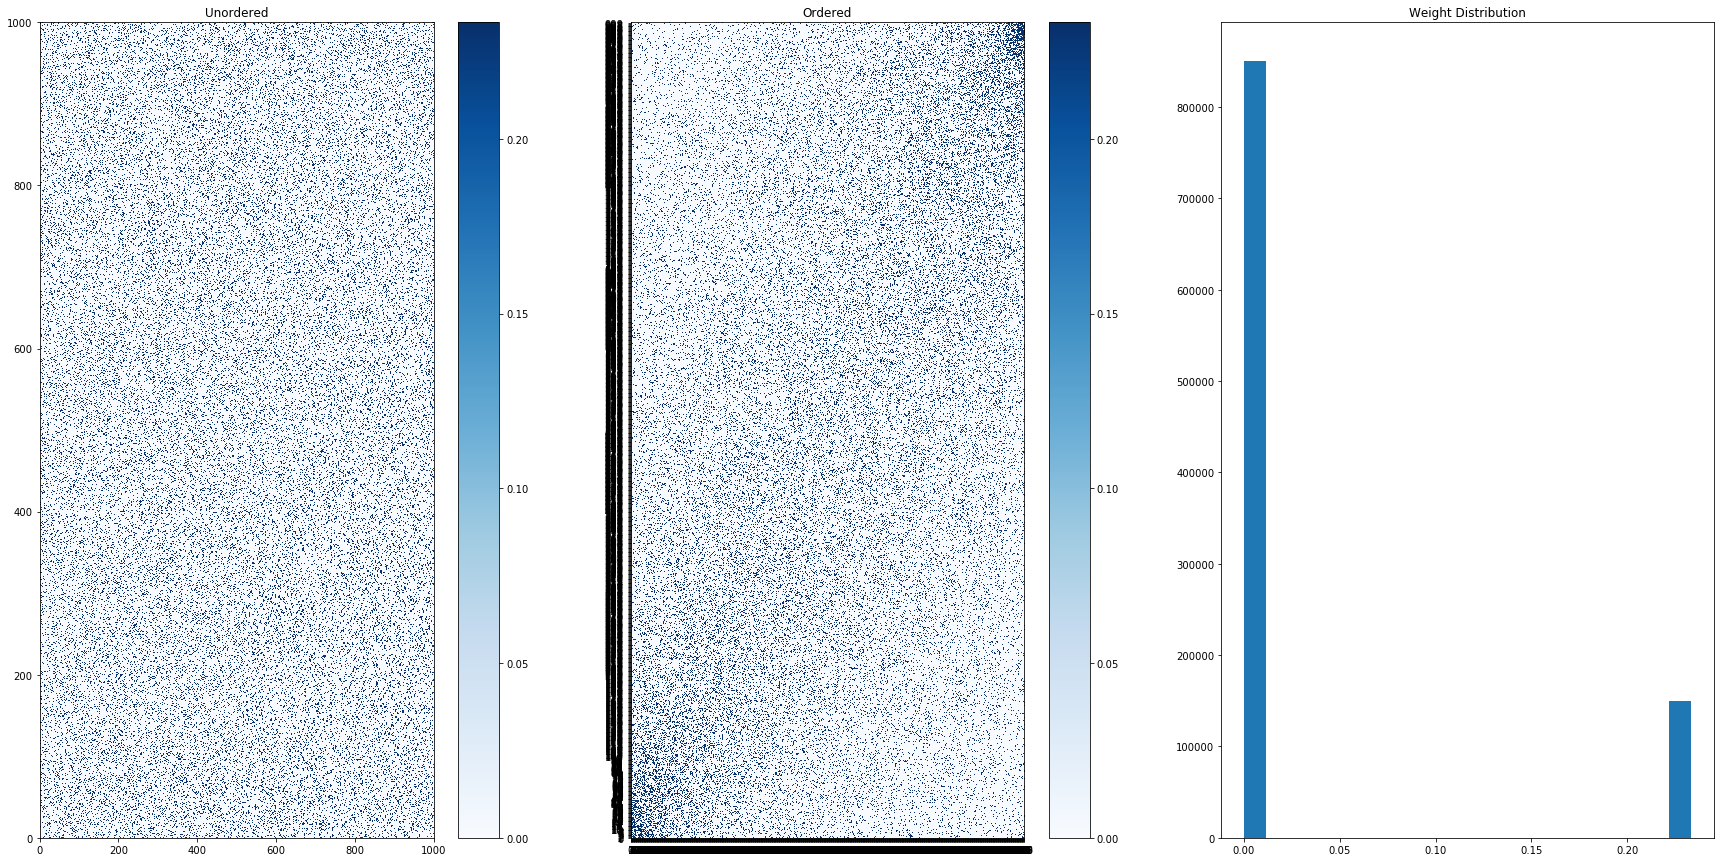
\includegraphics[width=1\linewidth,height=4cm]{/Users/sahand/Research/NeuroNet/Data/BW\s/N1000L\s00S\x D\y/Vis/Adjacency.png}
			\end{figure}

			\begin{figure}[H]
			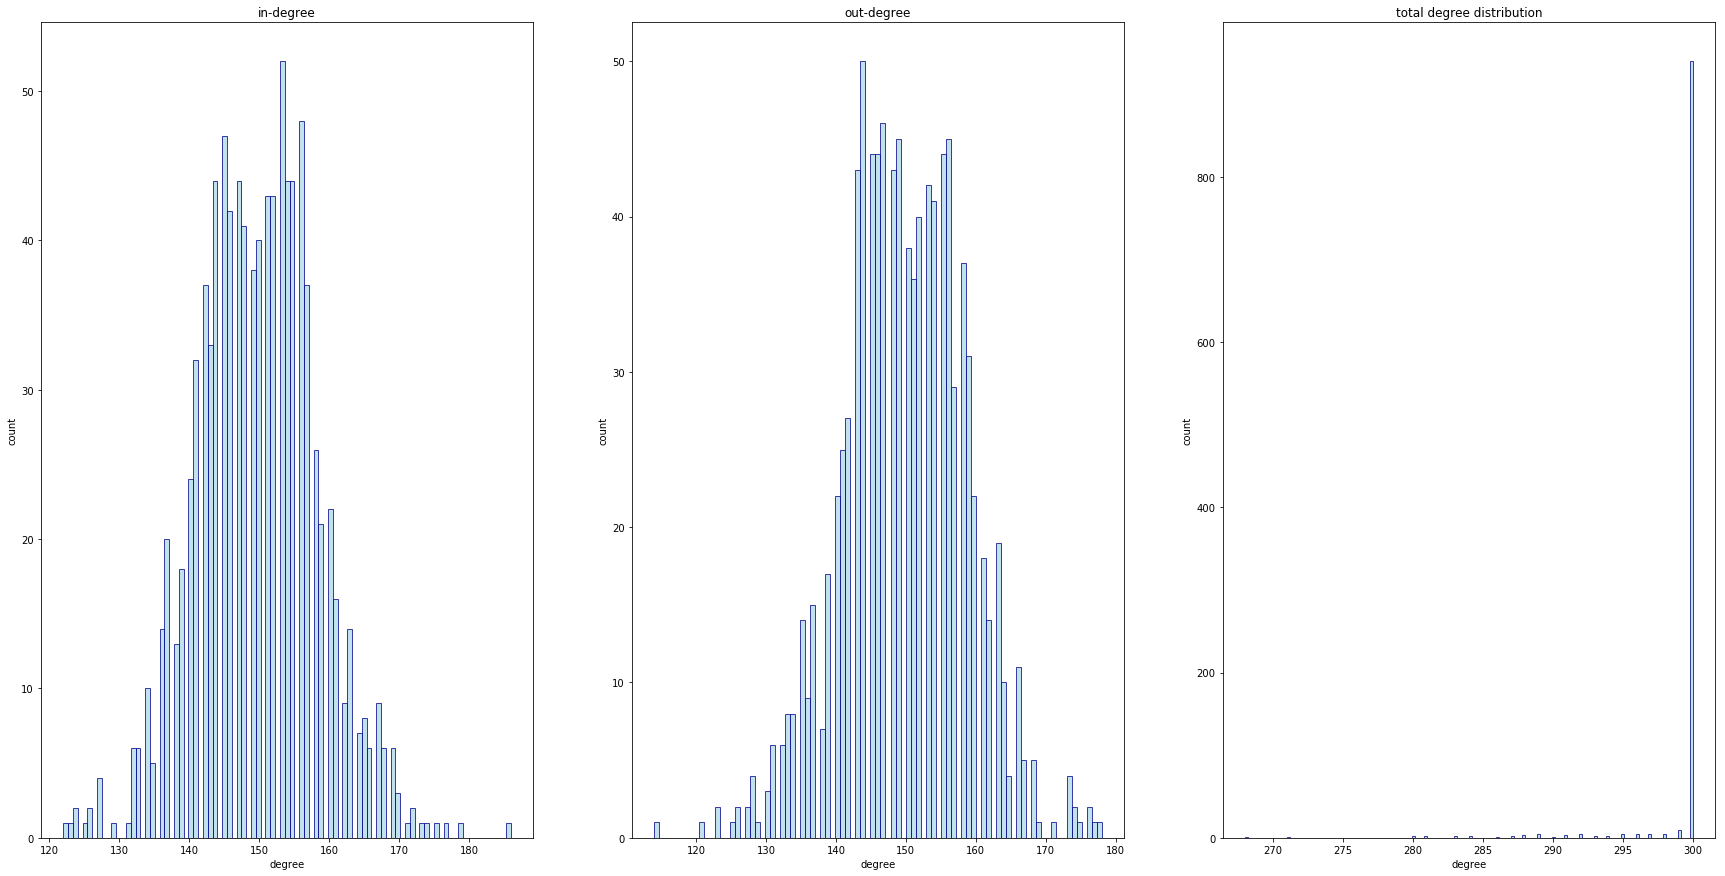
\includegraphics[width=1\linewidth,height=4cm]{/Users/sahand/Research/NeuroNet/Data/BW\s/N1000L\s00S\x D\y/Vis/DegreeDistribution.png}
			\end{figure}

			\pagebreak
			}
	}

}

\end{document}